\documentclass[a4paper,11pt]{scrartcl}
\usepackage{../packages/geosoftware}

\begin{document}

%Titelseite
\title{Geosoftware II \\ \small Feinplanung}
\author{Arndt, Autermann, Demuth, Fendrich, Ottenhues, Paluschek}
\date{\today}
\version{0.1}
\status{Entwurf}
\authormail{sloth@vespuccis.de}
%Titelseite wird Kreiert
\maketitle
\thispagestyle{empty}

\begin{center}
\bf Vers.: \MyVersion \\
\bf Stadium: \MyStatus\\
\bf Seiten: \thelastpage \\
\bf Kontakt: \email \\
\end{center}
\newpage

\tableofcontents

\newpage
%Ab gehts im Text

\section{Zielbestimmung}
	Die Zielbestimmungen sind dem Pflichtenheft in der aktuellsten Version zu entnehmen.\\

%\begin{samepage}	
\section{Verwendete Klassen}

\begin{landscape}
\begin{figure}[h]
\subsection{Klassendiagramm}
		\centering
		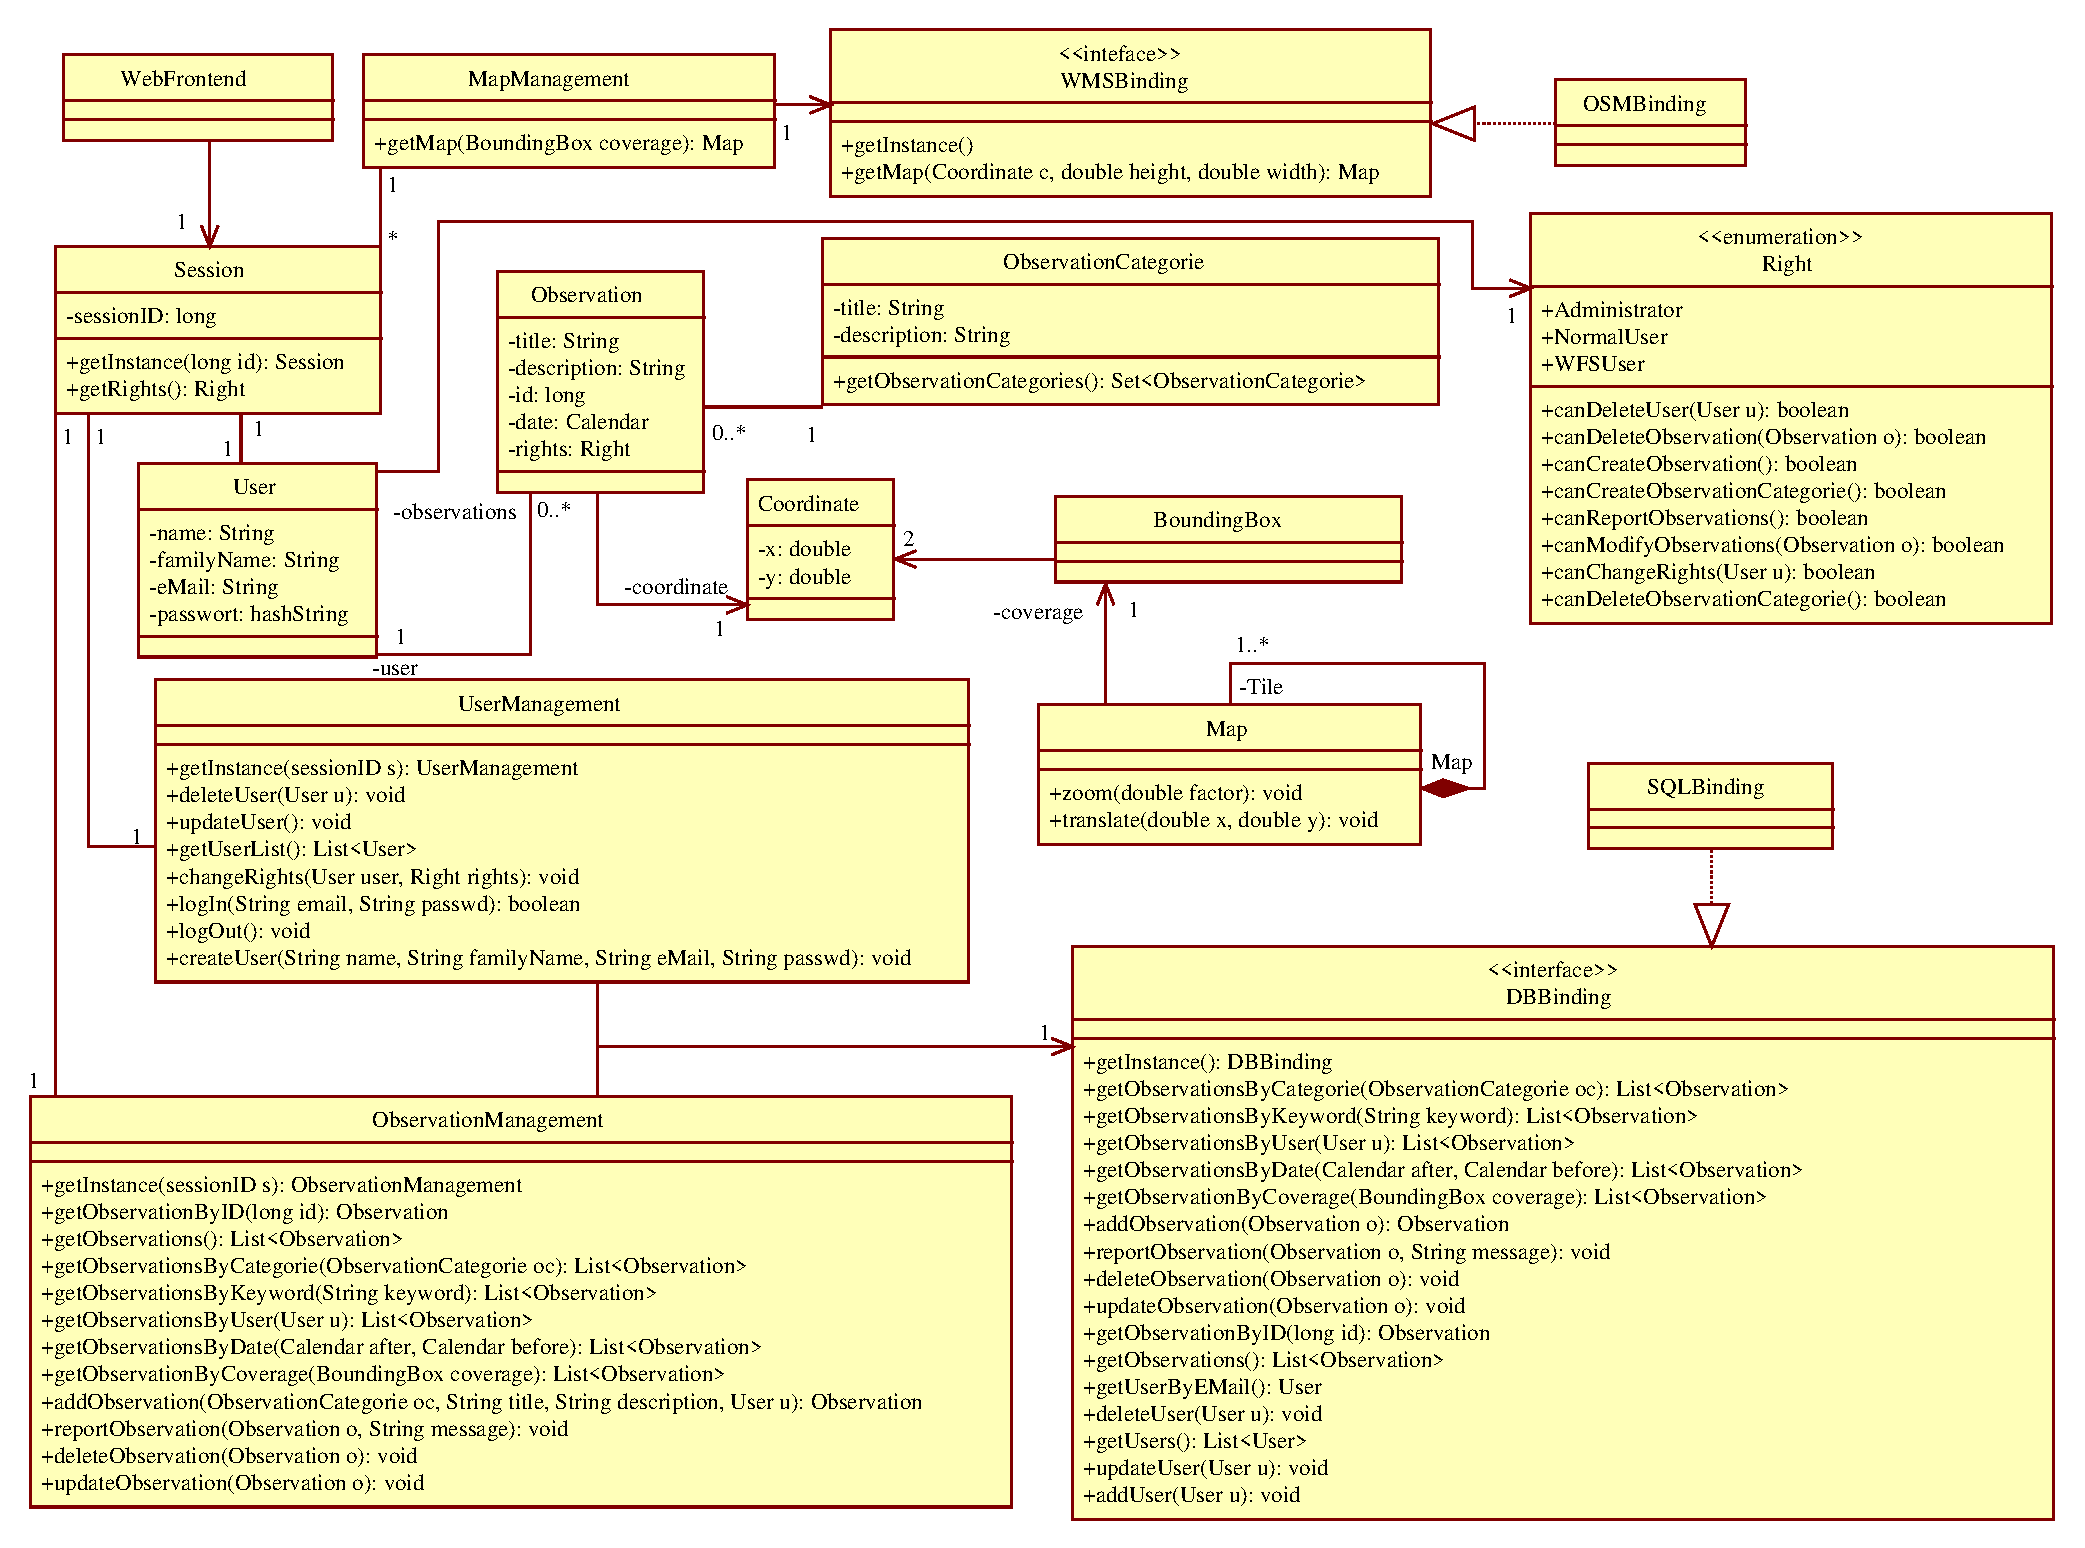
\includegraphics[width=0.90\textwidth]{images/classes.eps}
		\caption{Klassendiagramm des zu entwickelnden Systems}
		\label{Klassendiagramm}

\end{figure}
\end{landscape}
%\end{samepage}


\section{Sequenzen}
%\begin{samepage}
\begin{figure}[h]
\subsection{Einloggen}
		\centering
		\includegraphics[width=0.90\textwidth]{images/seq01_einloggen.eps}
		\caption{Sequenzieller Ablauf eines Anmeldevorgangs}
		\label{seq01}
\end{figure}
%\end{samepage}

%\begin{samepage}
\begin{figure}[h]
\subsection{Ausloggen}
		\centering
		\includegraphics[width=0.90\textwidth]{images/seq02_ausloggen.eps}
		\caption{Sequenzieller Ablauf eines Abmeldevorgangs}
		\label{seq02}
\end{figure}
%\end{samepage}


%\begin{samepage}
\begin{figure}[h]
\subsection{Konto Anlegen}
		\centering
		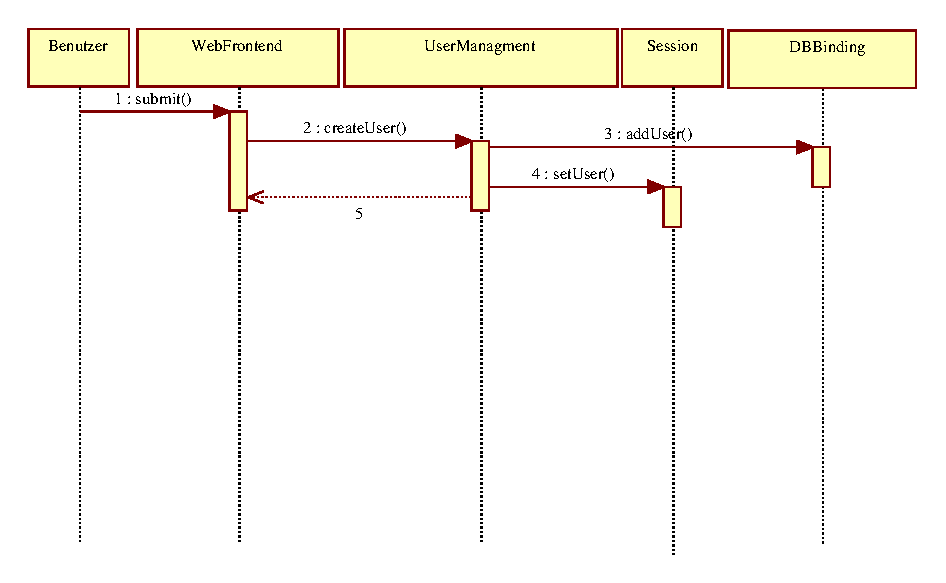
\includegraphics[width=0.90\textwidth]{images/seq03_KontoAnlegen.eps}
		\caption{Sequenzieller Ablauf eines KontoAnlegeVorganges}
		\label{seq03}
\end{figure}
%\end{samepage}


%\begin{samepage}
\begin{figure}[h]
\subsection{Konto Löschen}
		\centering
		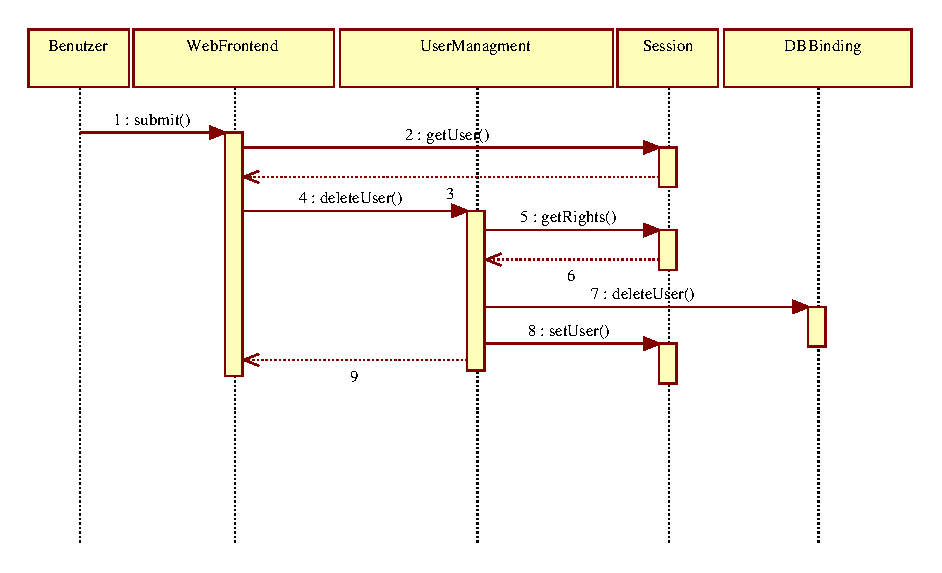
\includegraphics[width=0.90\textwidth]{images/seq04_KontoLoeschen.eps}
		\caption{Sequenzieller Ablauf eines KontoLoeschVorganges}
		\label{seq04}
\end{figure}
%\end{samepage}


%\begin{samepage}
\begin{figure}[h]
\subsection{Konto Details Einsehen}
		\centering
		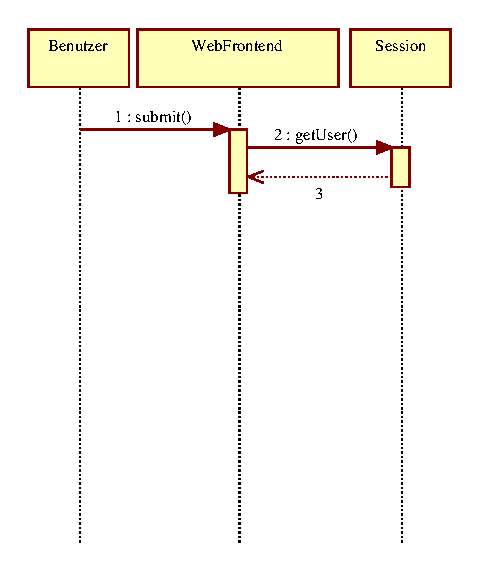
\includegraphics[width=0.90\textwidth]{images/seq05_KontoDetailsEinsehen.eps}
		\caption{Sequenzieller Ablauf eines Detail-Einseh-Vorganges}
		\label{seq05}
\end{figure}
%\end{samepage}


%\begin{samepage}
\begin{figure}[h]
\subsection{Konto Daten Ändern}
		\centering
		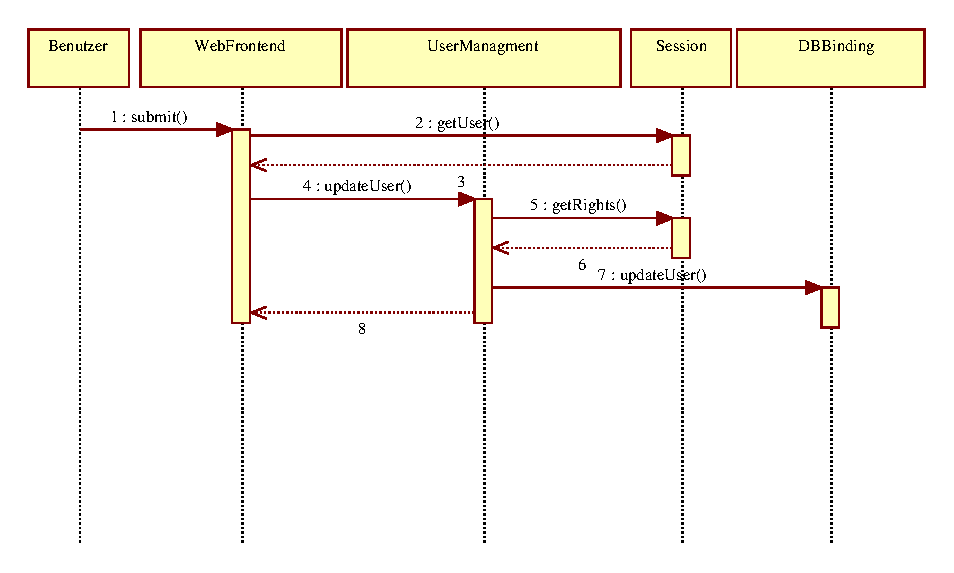
\includegraphics[width=0.90\textwidth]{images/seq06_KontoDatenAendern.eps}
		\caption{Sequenzieller Ablauf eines Aenderungsvorganges auf Konten}
		\label{seq06}
\end{figure}
%\end{samepage}


%\begin{samepage}
\begin{figure}[h]
\subsection{Ändern von Zugriffsrechten}
		\centering
		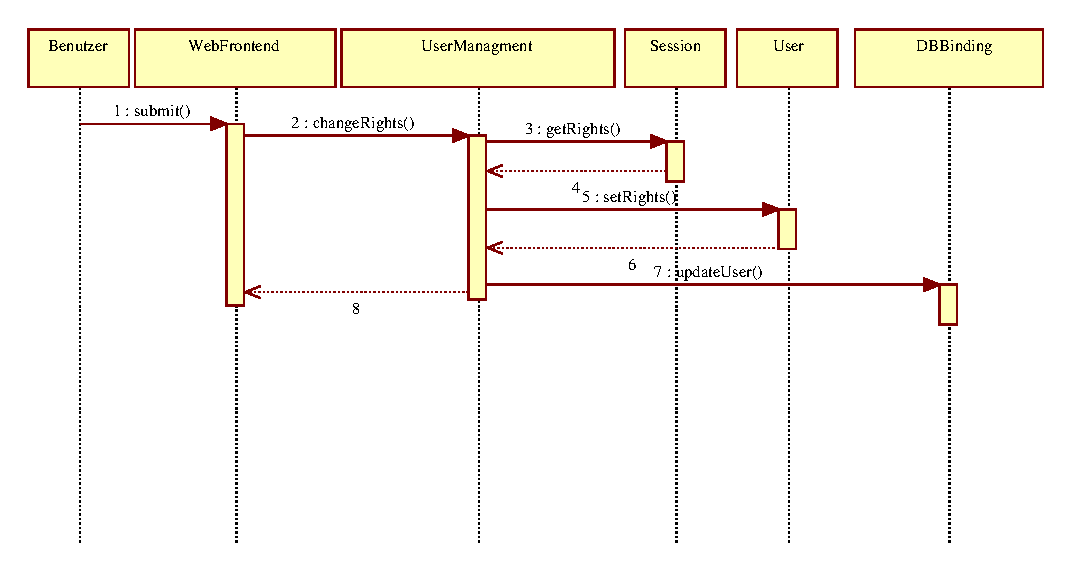
\includegraphics[width=0.90\textwidth]{images/seq07_KontoRechteAendern.eps}
		\caption{Sequenzieller Ablauf eines Rechteänderungsvorganges}
		\label{seq07}
\end{figure}
%\end{samepage}


%\begin{samepage}
\begin{figure}[h]
\subsection{Benutzerliste Anzeigen}
		\centering
		\includegraphics[width=0.90\textwidth]{images/seq08_benutzerlisteAnzeigen.eps}
		\caption{Sequenzieller Ablauf eines Benutzerliste Anzeigevorgangs}
		\label{seq08}
\end{figure}
%\end{samepage}


%\begin{samepage}
\begin{figure}[h]
\subsection{Ereignis eintragen}
		\centering
		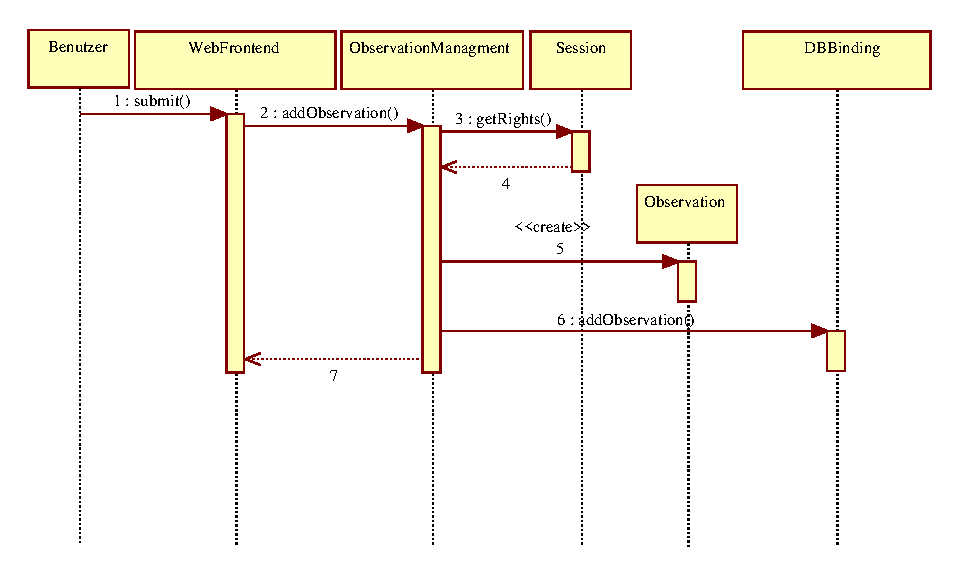
\includegraphics[width=0.90\textwidth]{images/seq09_EreignisEintragen.eps}
		\caption{Sequenzieller Ablauf eines Ereignis Eintragvorgangs}
		\label{seq02}
\end{figure}
%\end{samepage}


%\begin{samepage}
\begin{figure}[h]
\subsection{Ereignis einsehen}
		\centering
		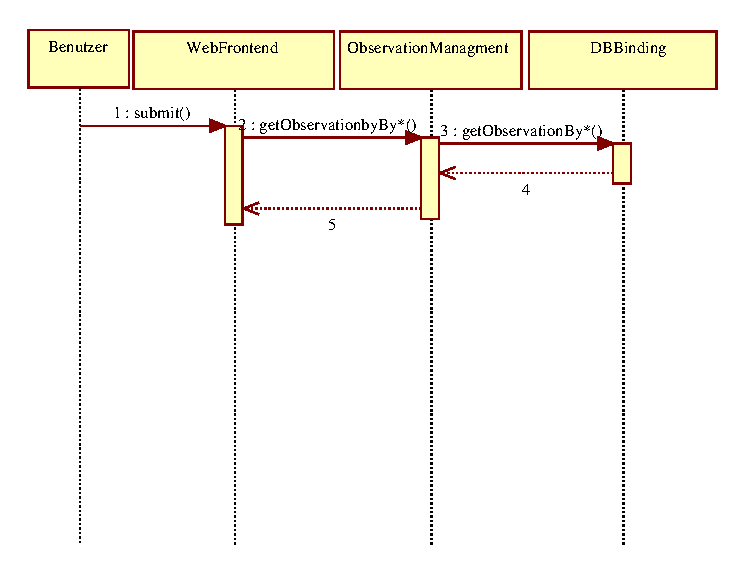
\includegraphics[width=0.90\textwidth]{images/seq10_EreignisEinsehen.eps}
		\caption{Sequenzieller Ablauf eines Eintrags Einsehenvorgangs}
		\label{seq10}
\end{figure}
%\end{samepage}



%\begin{samepage}
\begin{figure}[h]
\subsection{Ereignis ändern}
		\centering
		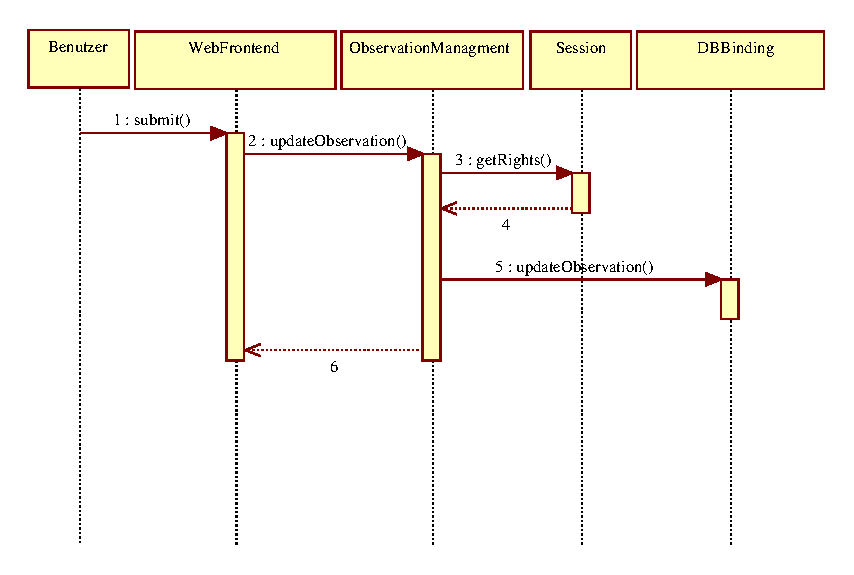
\includegraphics[width=0.90\textwidth]{images/seq11_EreignisAendern.eps}
		\caption{Sequenzieller Ablauf eines Ereignis Ändernvorgangs}
		\label{seq11}
\end{figure}
%\end{samepage}



%\begin{samepage}
\begin{figure}[h]
\subsection{Ereignis suchen}
		\centering
		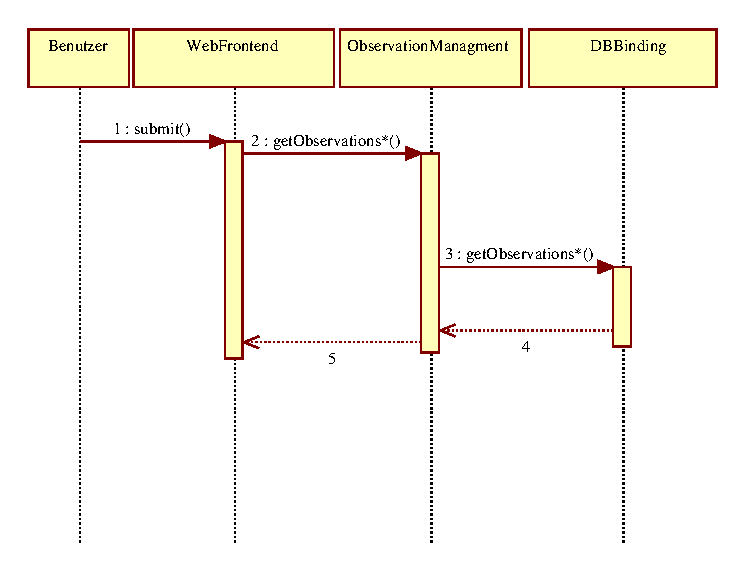
\includegraphics[width=0.90\textwidth]{images/seq12_EreignisSuchen.eps}
		\caption{Sequenzieller Ablauf eines Ereignis Suchvorgangs}
		\label{seq12}
\end{figure}
%\end{samepage}


%\begin{samepage}
\begin{figure}[h]
\subsection{Ereignis löschen}
		\centering
		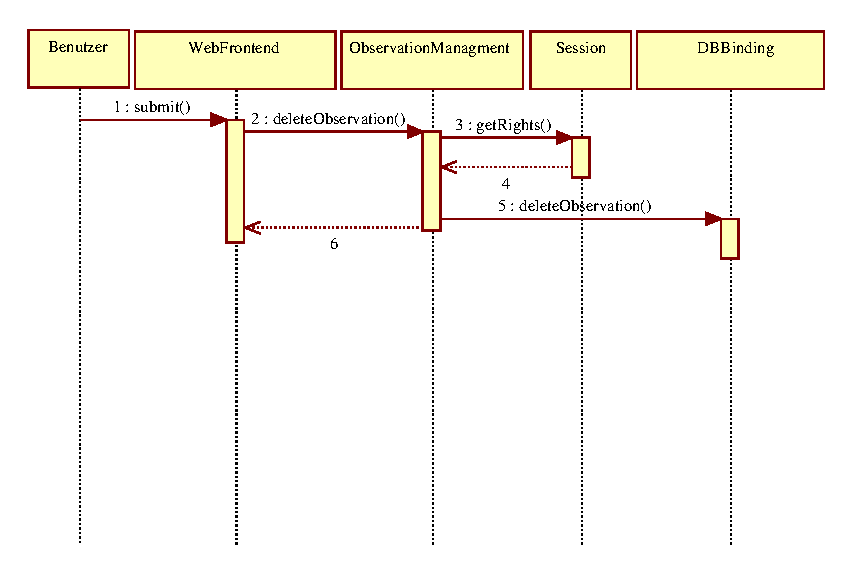
\includegraphics[width=0.90\textwidth]{images/seq13_EreignisLoeschen.eps}
		\caption{Sequenzieller Ablauf eines Ereignis Löschvorgangs}
		\label{seq13}
\end{figure}
%\end{samepage}



%\begin{samepage}

\begin{figure}[h]
\subsection{Ereignis melden}
		\centering
		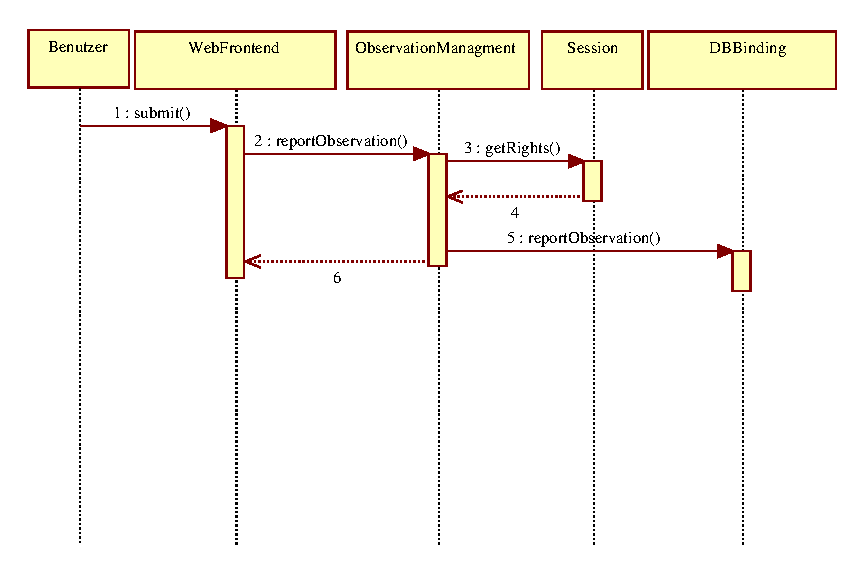
\includegraphics[width=0.90\textwidth]{images/seq14_EreignisMelden.eps}
		\caption{Sequenzieller Ablauf eines Ereignis Meldevorgangs}
		\label{seq14}
\end{figure}
%\end{samepage}


%\begin{samepage}
\begin{figure}[h]
\subsection{Karteninteraktion}
		\centering
		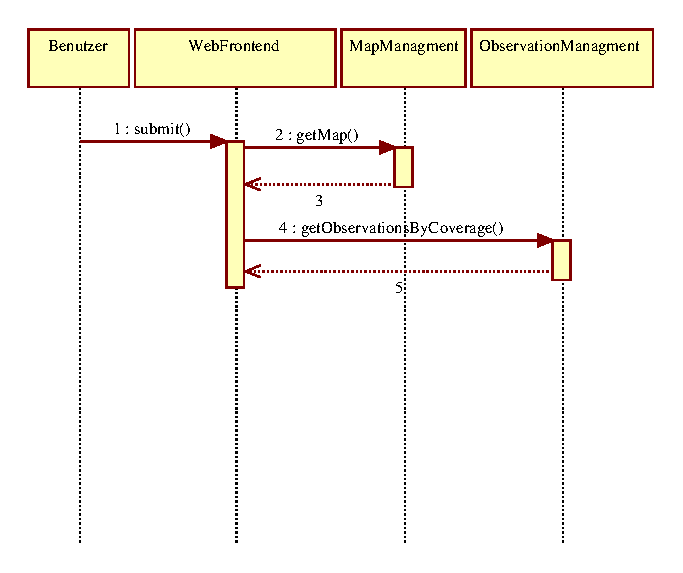
\includegraphics[width=0.90\textwidth]{images/seq15_KartenInteraktion.eps}
		\caption{Sequenzieller Ablauf eines Karten Interaktionsvorgangs}
		\label{seq15}
\end{figure}
%\end{samepage}
\end{document}
